\documentclass[a4paper,11pt]{article}
\usepackage[utf8]{inputenc}
\usepackage[T1]{fontenc}
\usepackage[french]{babel}
\usepackage{graphicx}
\usepackage{lipsum}
\usepackage[a4paper]{geometry}
\usepackage{wallpaper}
\usepackage{libertine}
\usepackage{csquotes}
\usepackage{fancyhdr}
\usepackage{vmargin}
\usepackage{hyperref}
\usepackage[colorinlistoftodos]{todonotes}
\usepackage{titlesec}
\usepackage{array}

\pagestyle{fancy}

\makeatletter
\def\clap#1{\hbox to 0pt{\hss #1\hss}}%
\def\ligne#1{%
\hbox to \hsize{%
\vbox{\centering #1}}}%
\def\haut#1#2#3{%
\hbox to \hsize{%
\rlap{\vtop{\raggedright #1}}%
\hss
\clap{\vtop{\centering #2}}%
\hss
\llap{\vtop{\raggedleft #3}}}}%
\def\bas#1#2#3{%
\hbox to \hsize{%
\rlap{\vbox{\raggedright #1}}%
\hss
\clap{\vbox{\centering #2}}%
\hss
\llap{\vbox{\raggedleft #3}}}}%
\def\maketitle{%
\thispagestyle{empty}\vbox to \vsize{%
\haut{}{\@blurb}{}
\vfill
\vspace{1cm}
\begin{flushleft}
\usefont{OT1}{ptm}{m}{n}
\huge \@title
\end{flushleft}
\par
\hrule height 4pt
\par
\begin{flushright}
\usefont{OT1}{phv}{m}{n}
\Large \@author
\par
\end{flushright}
\vspace{1cm}
\vfill
\vfill
\bas{}{\@location, le \@date}{}
}%
\cleardoublepage
}
\def\date#1{\def\@date{#1}}
\def\author#1{\def\@author{#1}}
\def\title#1{\def\@title{#1}}
\def\location#1{\def\@location{#1}}
\def\blurb#1{\def\@blurb{#1}}
\Large{\date{\today}}
\author{}
\title{}
\location{Rennes}\blurb{}
\makeatother
\title{\LARGE{Projet Modélisation et Programmation Orientée Objet}}
\author{Frank \textsc{Chassing} et Amandine \textsc{Fouillet}}
\location{Rennes}
\blurb{%
\large{INSA de Rennes\\
\textbf{Rapport de conception}}
}%

%En-têtes
\renewcommand{\headrulewidth}{0.5pt}
\fancyhead[L]{\textit{\leftmark}}
\fancyhead[C]{}
\fancyhead[R]{}

\begin{document}
\maketitle
\tableofcontents
\newpage

\section*{Introduction}
	\addcontentsline{toc}{section}{Introduction}
	Dans le cadre des cours de Programmation Orientée Objets et de Modélisation et Conception de Logiciels, nous sommes amenés à réaliser un jeu pour ordinateur semblable au jeu Small World. Ce projet se déroule en deux temps : dans la première partie nous avons réalisé la modélisation du problème grâce à divers diagrammes UML puis, dans la seconde partie, nous réaliserons l'implémentation du jeu. \\

	Le jeu à réaliser est un jeu tour à tour dans lequel chaque joueur dirige un peuple qui contient plusieurs unités. Le but du jeu est de gérer les unités sur une carte du monde pour obtenir le plus de points possible à la fin d'un certain nombre de tours. Pour gagner il faut contrôler le plus de cases possible en attaquant les unités adverses, en défendant son territoire et en se déplaçant sur les cases vides. Dans notre implémentation du jeu, deux joueurs s'opposeront, ils pourront choisir trois peuples différents : les Elfs, les Orcs et les Nains et se déplacer sur trois types de cases différents : la forêt, le désert, la montagne et la plaine.\\

	Ce rapport présente le travail réalisé lors de la phase de modélisation au cours de laquelle plusieurs diagrammes ont été réalisés afin de décrire les différents aspects du jeu. Ainsi, dans un premier temps nous étudierons la phase de création d'une partie grâce aux diagrammes de cas d'utilisation, d'activité et de séquence. Puis nous étudierons le déroulement d'une partie, d'un tour de jeu et d'un combat là encore avec des diagrammes d'interaction, d'activité et de cas d'utilisation. Pour résumer et conclure sur la modélisation du jeu, nous finirons par détailler le diagramme de classes réalisé ainsi que les différents patrons de conception utilisés.
	\newpage

\section{Création de la partie}
	\vspace*{0.5cm}
	Commençons par détailler ce qui se passe lors de l'ouverture du jeu. Lors de la création d'une nouvelle partie, l'utilisateur commence par choisir une carte parmi les trois différents types (la démo, la petite et la normale). C'est ce choix de carte qui détermine le nombre de cases et le nombre de tours, elle est créée de manière aléatoire. Pour pouvoir jouer, il est nécessaire que les joueurs soient au nombre de deux, ils sont créés après le choix de la carte. Les deux joueurs doivent choisir un pseudo et un peuple différent (Elf, Nain ou Orc). Une fois ces tâches réalisées, la partie peut commencer. Si une partie précédente avait été abandonnée avant la fin du jeu, lors de l'ouverture les joueurs peuvent choisir de reprendre cette ancienne partie ou en commencer une nouvelle.  De même, de façon évidente, l'utilisateur peut abandonner la création de la partie à tout moment en quittant le jeu. 
	\vspace*{0.5cm}
	
	\subsection{Diagramme de cas d'utilisation}
		\vspace*{0.5cm}
		\begin{figure}[h!]
			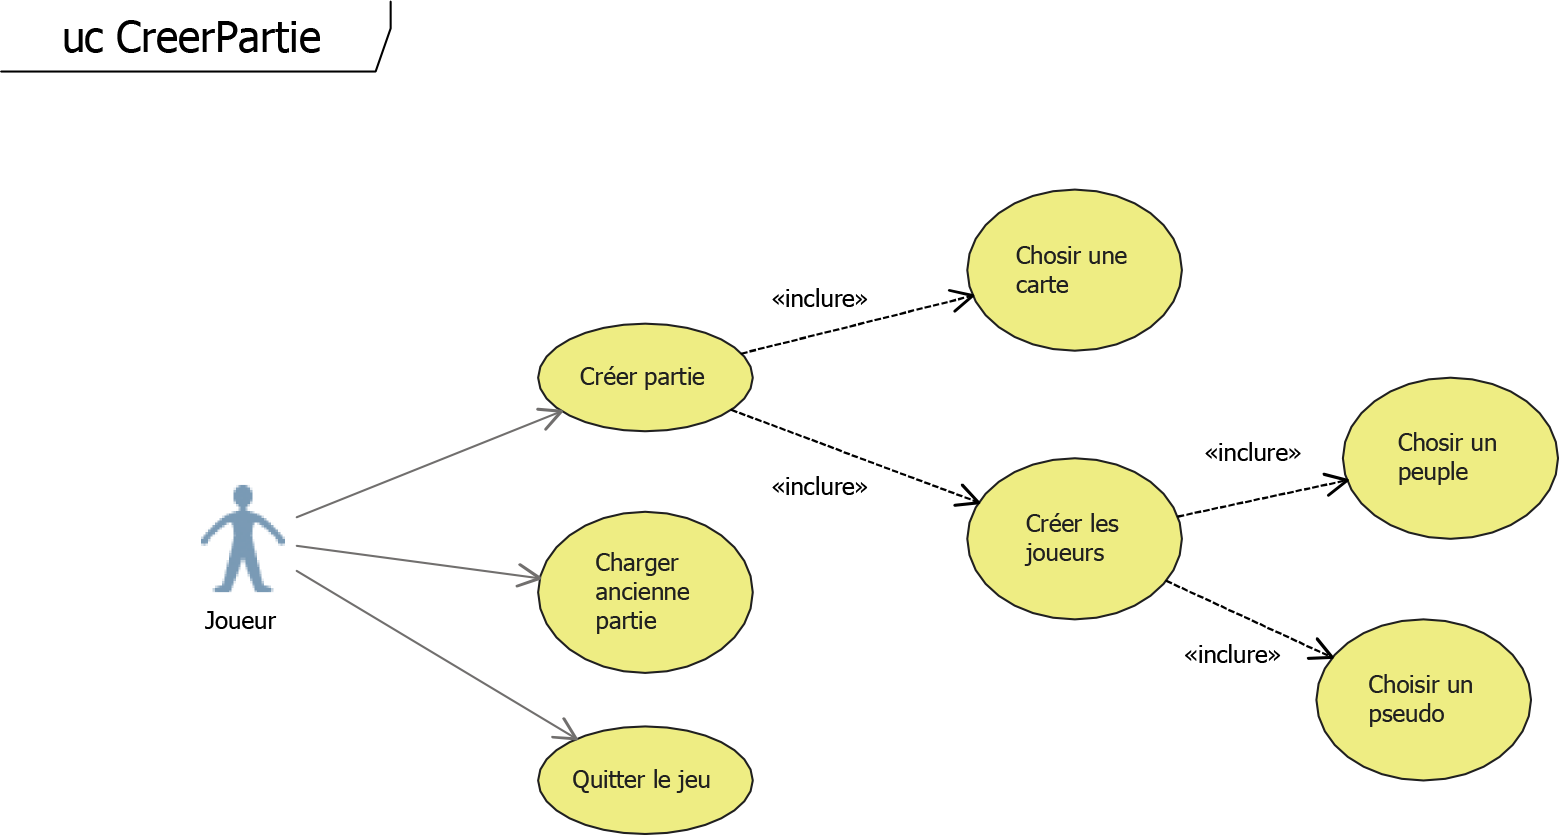
\includegraphics{ucCreerPartie.png}
			\caption{Diagramme de cas d'utilisation - Créer une partie}
			\label{fig:uccreer}
		\end{figure}
		\vspace*{1cm}
		Le diagramme de cas d'utilisation ci-dessus (\textsc{Figure \ref{fig:uccreer}}) illustre la création d'une partie du point de vue utilisateur. En arrivant sur l'interface d'accueil du jeu le joueur a trois possibilités : créer une nouvelle partie, charger une ancienne partie ou quitter l'application. Si l'utilisateur décide de créer une nouvelle partie, il commence par choisir une carte puis il crée les deux joueurs en donnant à chacun un pseudo et un peuple.
		\newpage

	\subsection{Diagramme d'activité}
		\vspace*{0.5cm}
		\begin{figure}[ht!]
			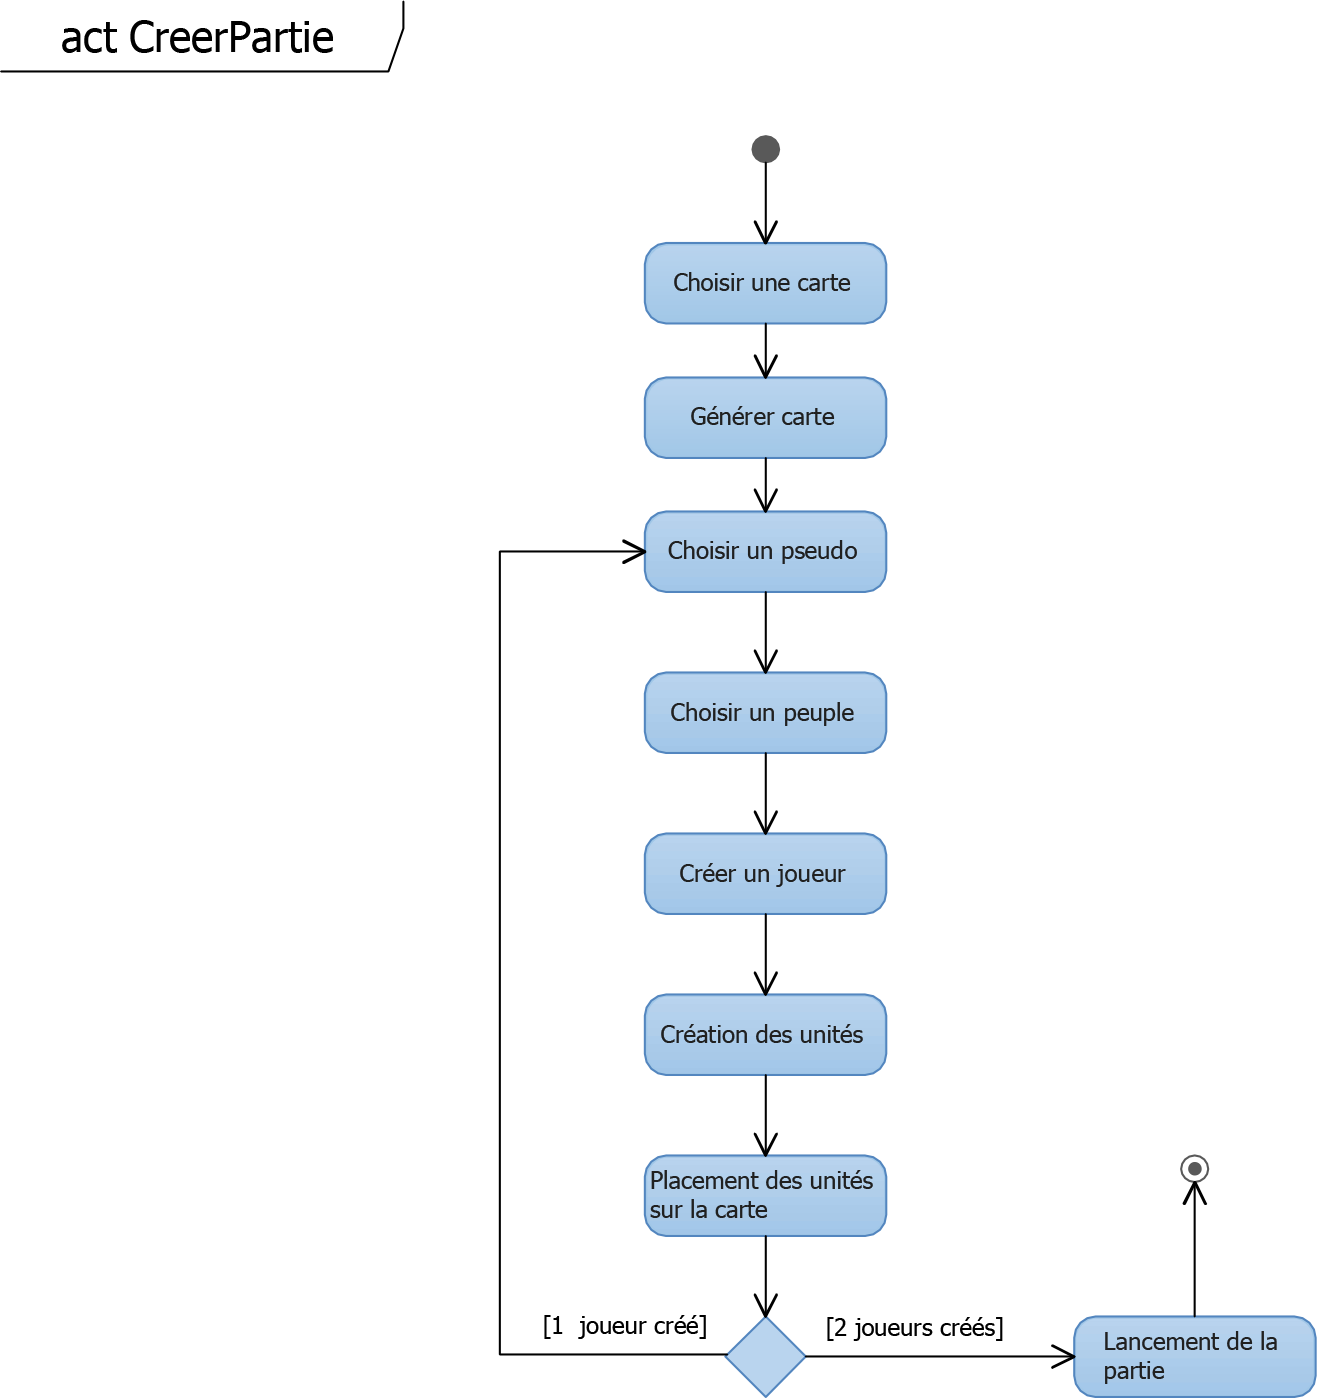
\includegraphics{actCreerPartie.png}
			\caption{Diagramme d'activité - Créer une partie}
			\label{fig:actcreer}
		\end{figure}
		\vspace*{1cm}
		Le diagramme d'activité ci-dessus (\textsc{Figure \ref{fig:actcreer}}) illustre le processus de création d'une partie. Lorsque le système est en état de création d'une partie, l'évènement permettant à l'utilisateur de choisir une carte est le premier à se déclencher. Ensuite, le système rentre dans un processus de création d'un joueur : choix d'un pseudo, choix d'un peuple, création du joueur puis placement des unités sur la carte. À la fin du processus de création d'un joueur, le système vérifie le nombre de joueurs déjà créés : s'il n'y a qu'un joueur créé on retourne au début du processus de création d'un joueur, s'ils sont deux on lance la partie.
		\newpage

	\subsection{Diagramme de séquence}
		\begin{figure}[ht!]
			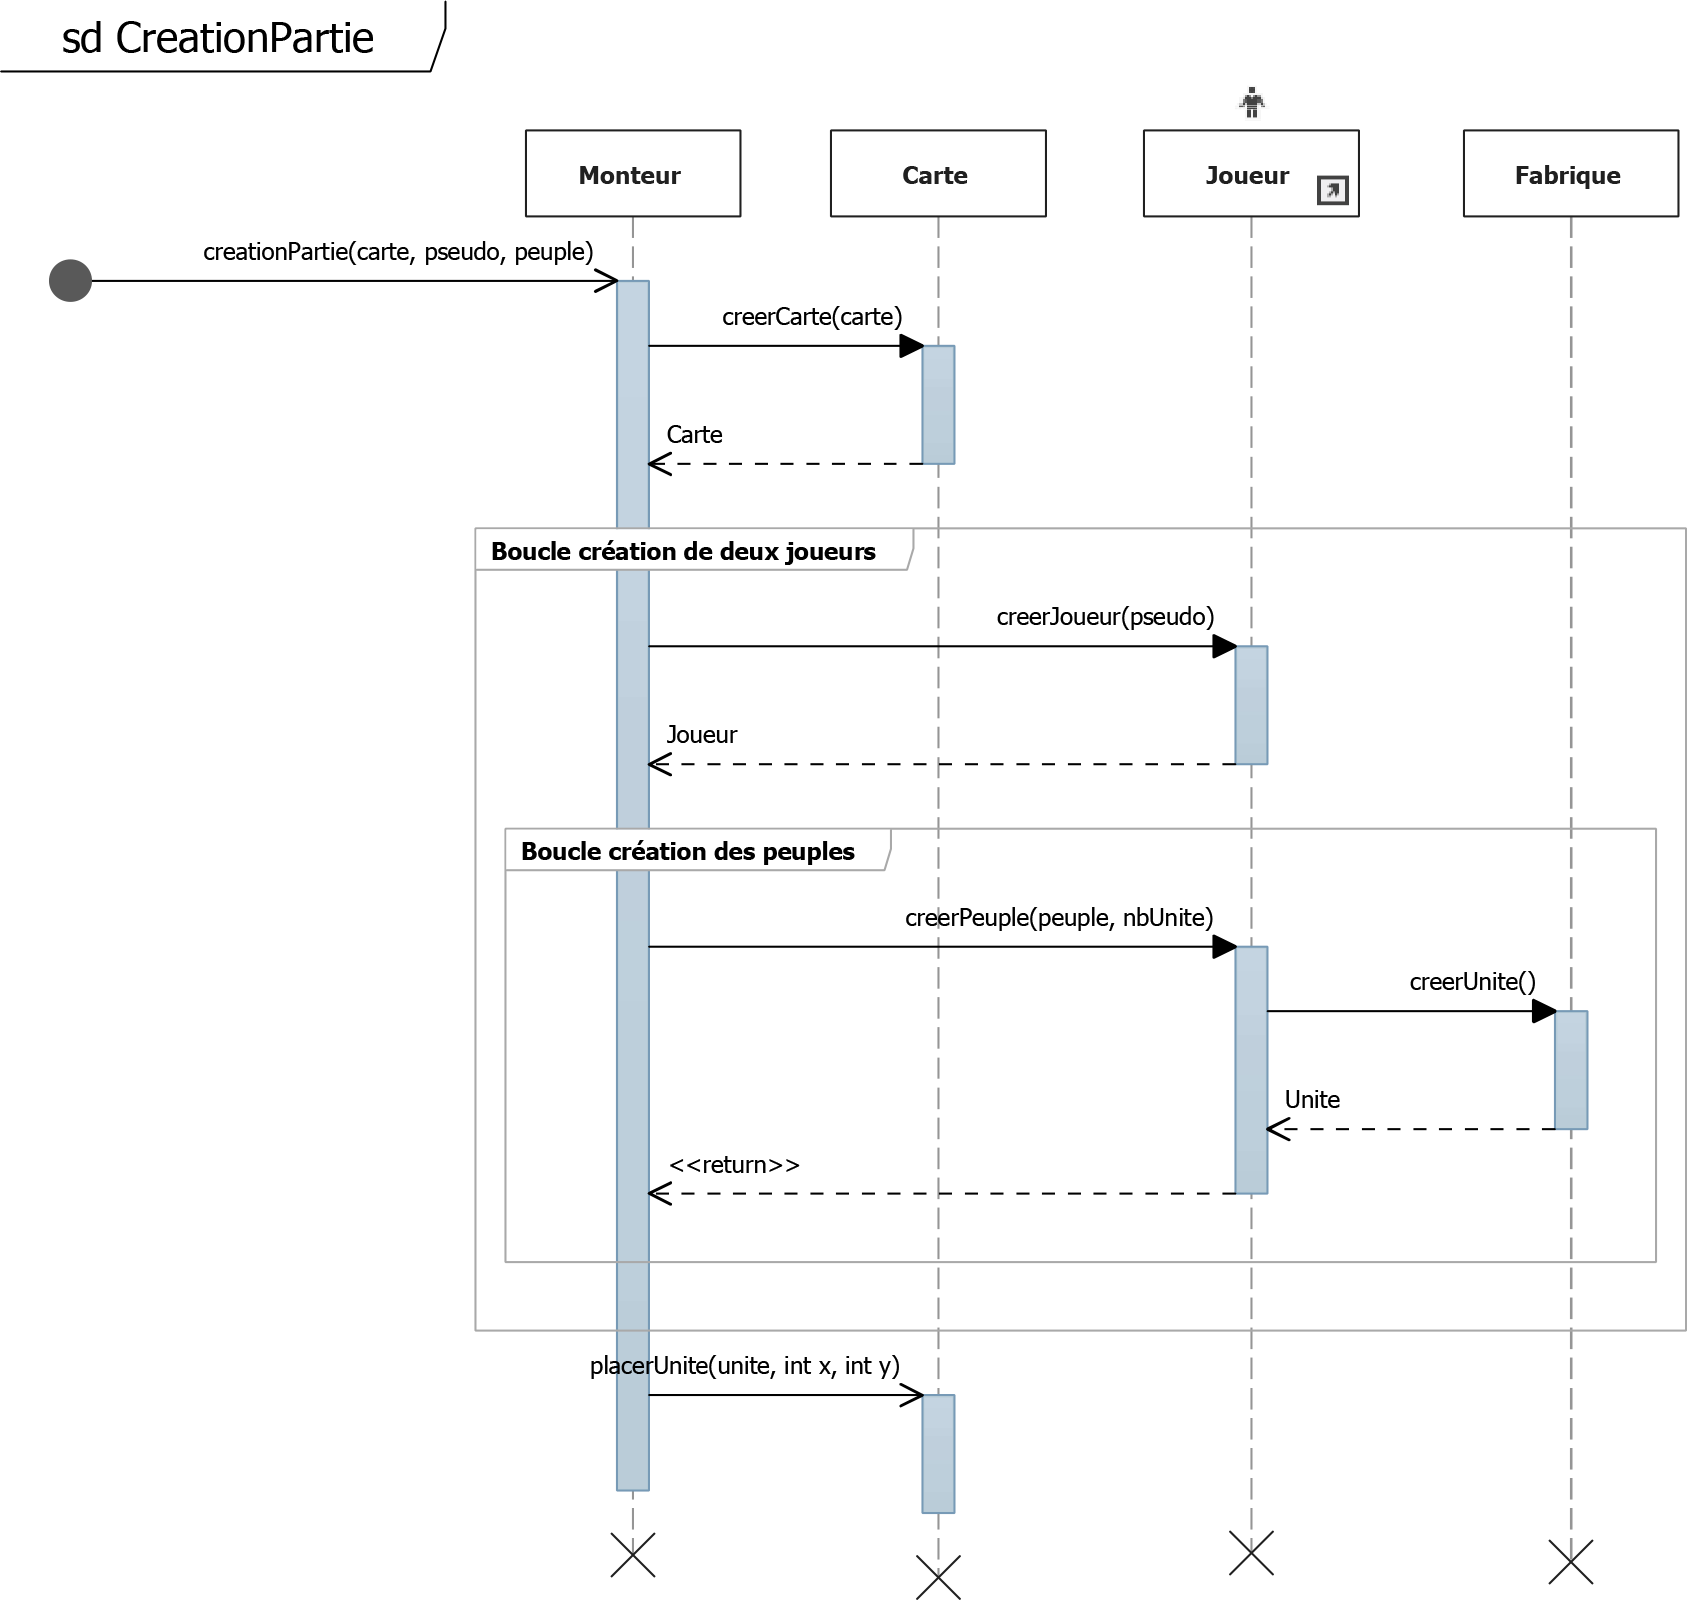
\includegraphics[height=17cm]{sqCreerPartie.png}
			\caption{Diagramme de séquence - Créer une partie}
			\label{fig:seqcreer}
			\end{figure}
		\vspace*{1cm}
		Le diagramme de séquence ci-dessus (\textsc{Figure \ref{fig:seqcreer}}) illustre les interactions entre objets lors de la création d'une partie. On observe les mêmes événements qu'avec le diagramme d'activité mais, en étudiant la dimension temporelle, on met en évidence des boucles de création. En effet, le monteur crée deux joueurs à qui il attribue deux peuples différents. Chaque peuple crée ensuite ses unités que le monteur place sur la carte.
		\newpage 

\section{Déroulement d'une partie}
	\vspace*{0.5cm}
	Une fois que la partie est lancée, l'ordre de jeu est choisi aléatoirement et un des deux joueurs commence à jouer. Le déroulement d'un tour de jeu est décrit dans la suite de ce rapport. Un des joueurs peut perdre ses unités durant le tour, la partie s'arrête alors et l'autre joueur gagne. À la fin du nombre de tours, si aucun joueur n'a perdu avant, on calcule le nombre de points de chaque joueur pour déterminer le vainqueur. Le diagramme d'activité ci-dessous (\textsc{Figure \ref{fig:actpartie}}) illustre le processus de déroulement d'une partie. L'état "Lancement de la partie" a été détaillé dans le diagramme d'activité de création d'une partie tandis que l'état "Tour du joueur" sera détaille par la suite.

	\vspace*{1cm}
	\begin{figure}[ht!]
		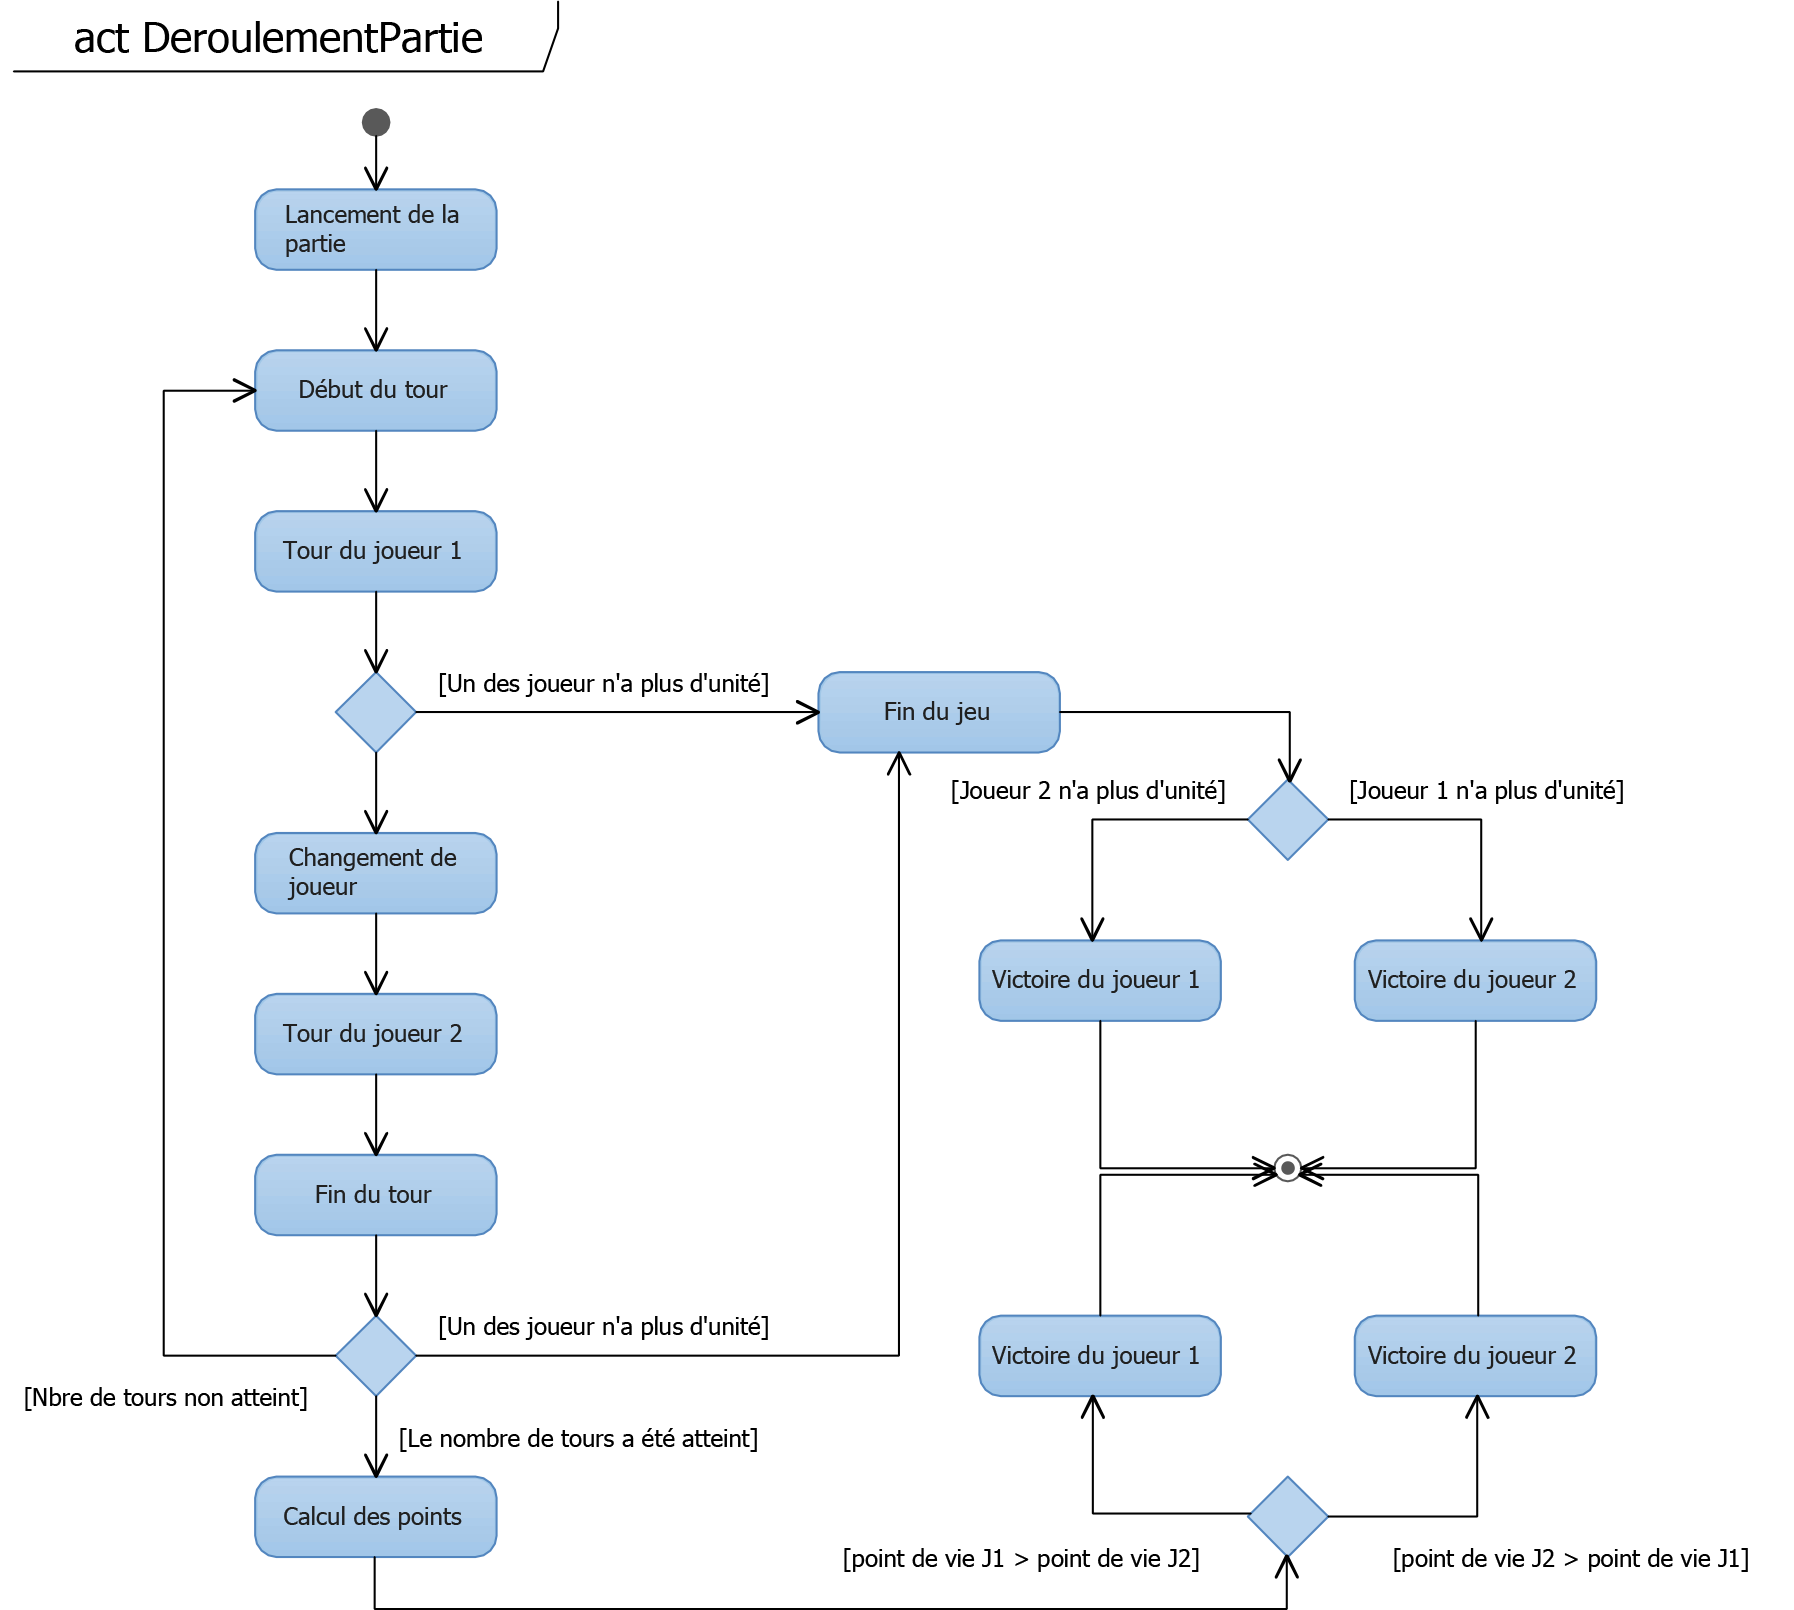
\includegraphics{actDeroulementPartie.png}
		\caption{Diagramme d'activité - Déroulement d'une partie}
		\label{fig:actpartie}
	\end{figure}
	\vspace*{1cm}
	\newpage

	\subsection{Déroulement d'un tour de jeu}
		\vspace*{0.5cm}
		Lorsqu'un joueur peut jouer, il peut déplacer toutes chacune des unités suivant son nombre de points de mouvement ou choisir de passer son tour. Une unité combattante peut engager un combat si elle se déplace sur une case ennemie. Lorsqu'un joueur à finit son tour, il clique sur le bouton "Fin du tour". Le tour peut cependant être arrêté prématurément si un des joueurs perd un combat et n'a plus d'unité, le jeu se termine alors.
		\vspace*{0.5cm}

		\subsubsection{Diagramme de cas d'utilisation}
			\begin{figure}[ht!]
				\includegraphics{ucTourDeJeu.png}
				\caption{Diagramme de cas d'utilisation - Déroulement d'un tour de jeu}
				\label{fig:uctour}
			\end{figure}
			\vspace*{1cm}
			Le diagramme de cas d'utilisation ci-dessus (\textsc{Figure \ref{fig:uctour}}) illustre le déroulement d'un tour de jeu du point de vue utilisateur. Lorsque c'est à son tour de jouer, l'utilisateur doit choisir une action pour chacune de ses unités. Il a la possibilité de ne rien faire, déplacer l'unité dans une case vide ou d'attaquer le peuple ennemi. À  tout moment, le joueur peut décider de finir le tour ou de quitter la partie.
			\newpage

		\subsubsection{Diagramme d'activités}
			\begin{figure}[ht!]
				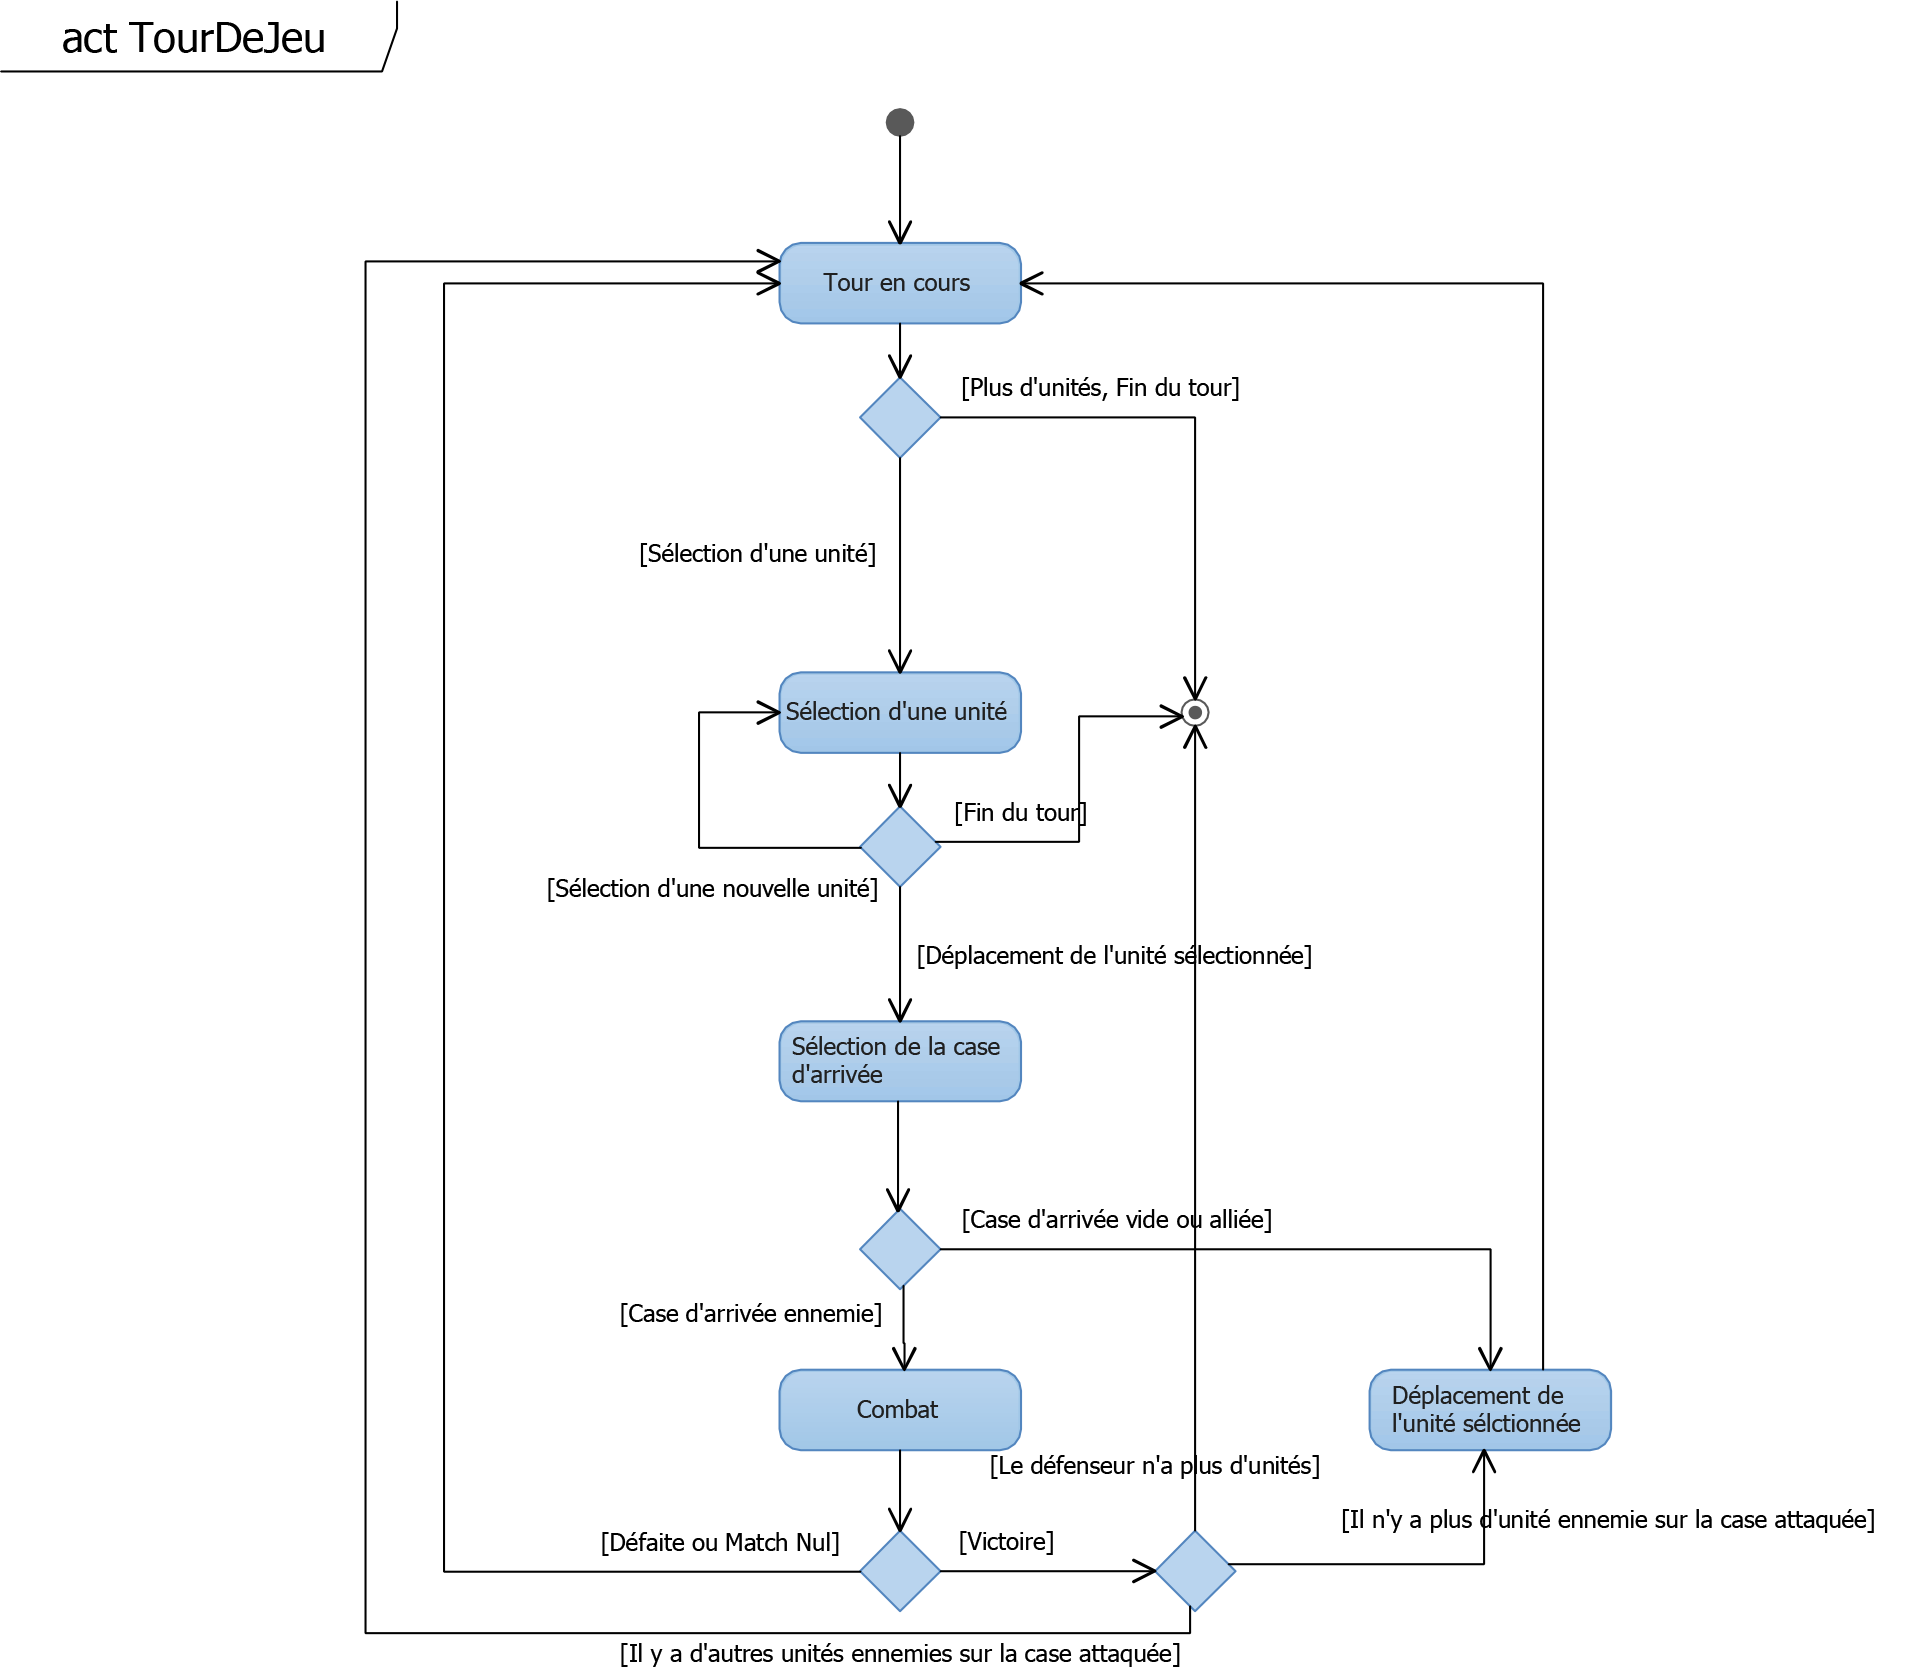
\includegraphics{actTourDeJeu.png}
				\caption{Diagramme d'activité - Déroulement d'un tour de jeu}
				\label{fig:acttour}
				\end{figure}
			\vspace*{1cm}
			Le diagramme d'activité ci-dessus (\textsc{Figure \ref{fig:acttour}}) illustre le processus du déroulement d'un tour de jeu. Un tour est en cours, si le joueur n'appuie pas sur le bouton "Fin du tour", il doit sélectionner une unité. Il y a alors deux possibilités : soit l'unité passe son tour et on en sélectionne une nouvelle, soit l'unité se déplace. Si l'unité se déplace, on doit sélectionner la case d'arrivée. Si cette case d'arrivée est vide ou alliée, on déplace l'unité sélectionnée, sinon, un combat se déroule. En cas de défaite ou de match nul, on revient au début du processus tour de jeu si le joueur n'a plus d'unité pour continuer le jeu ou s'il décide d'arrêter, le tour est fini, sinon, on retourne dans le processus de sélection d'une unité. D'un autre côté, si l'unité gagne et s'il n'y a plus d'unité dans la case attaquée elle est déplacée sur cette case.
			\newpage

		\subsubsection{Diagramme de séquence}
			\begin{figure}[ht!]
				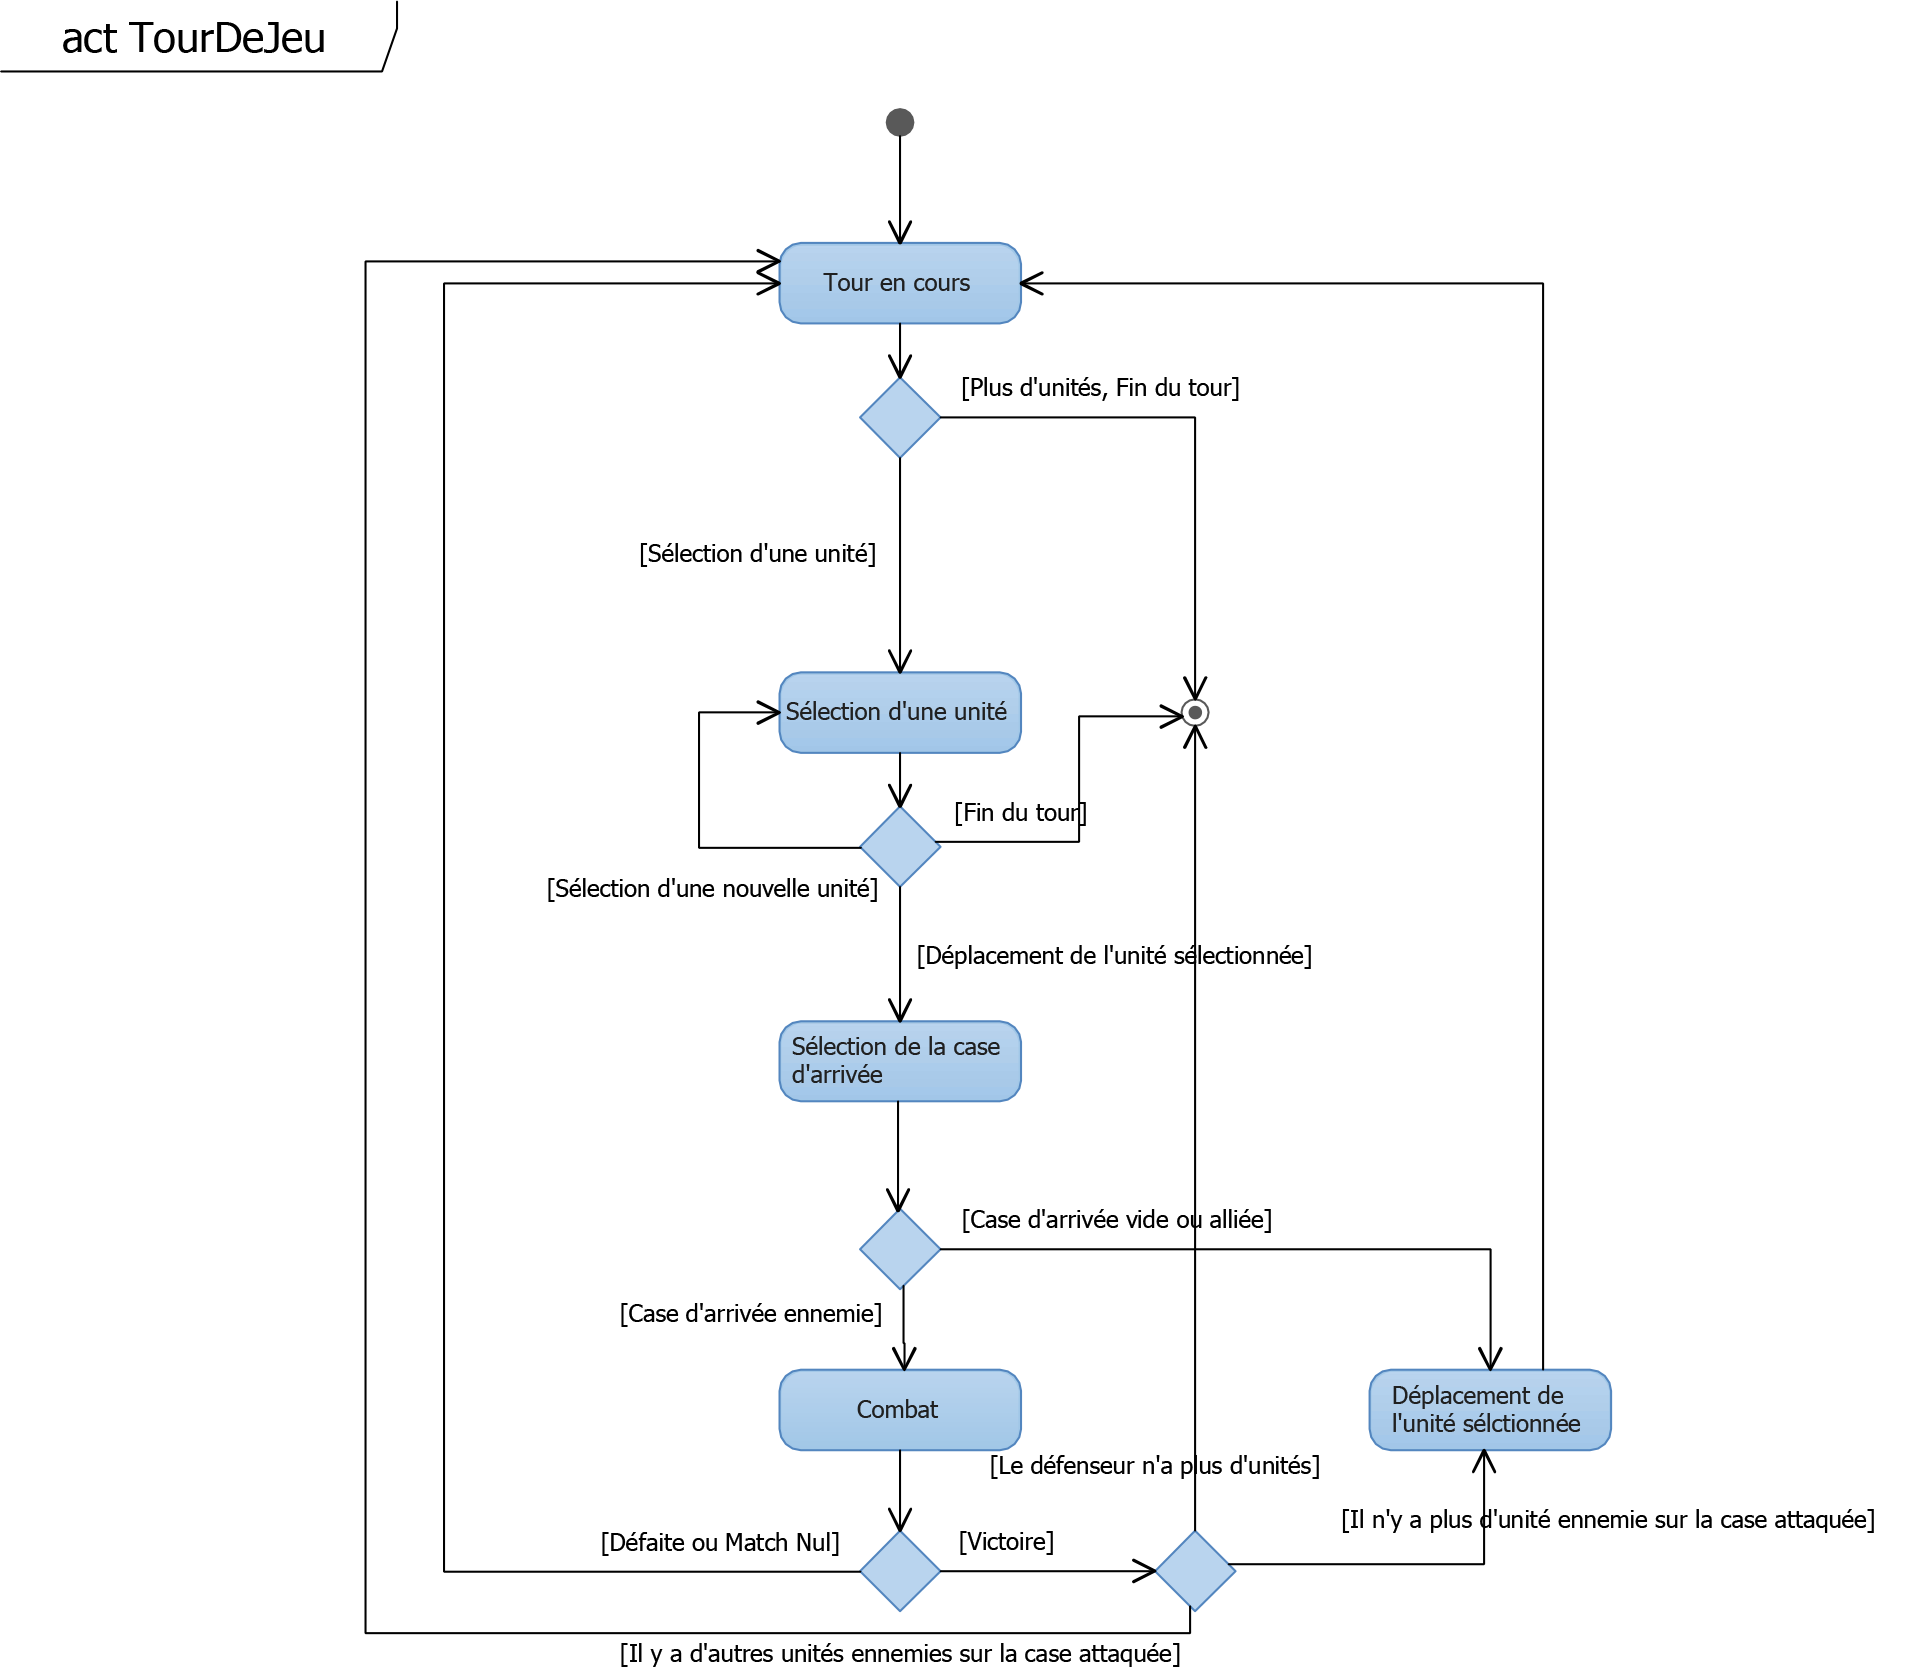
\includegraphics{actTourDeJeu.png}
				\caption{Diagramme de séquence - Déroulement d'un tour de jeu}
				\label{fig:seqtour}
				\end{figure}
			\vspace*{1cm}
			Le diagramme de séquence ci-dessus (\textsc{Figure \ref{fig:seqtour}}) illustre les interactions entre objets lors du déroulement d'une partie.
			\newpage

		\subsubsection{Diagramme d'état transition}
			\begin{figure}[ht!]
				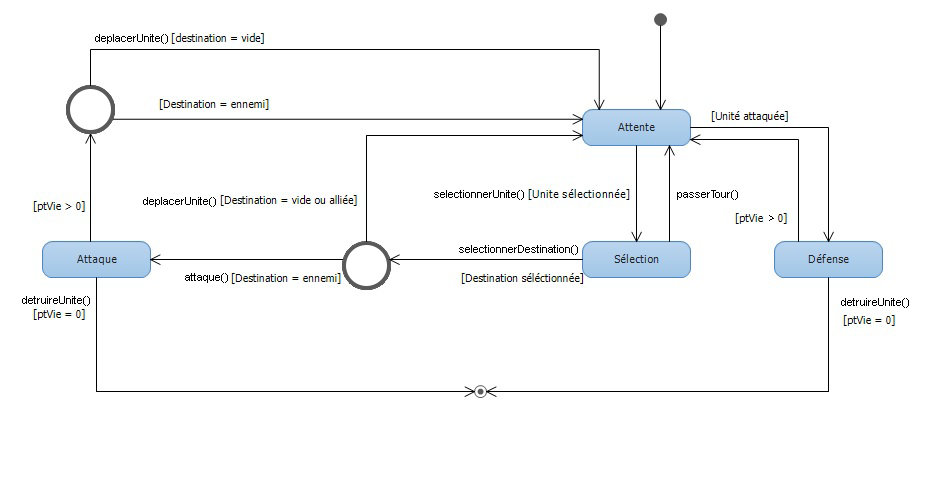
\includegraphics[width=15cm]{ettour.png}
				\caption{Diagramme d'état transition- Déroulement d'un tour de jeu}
				\label{fig:ettour}
				\end{figure}
			\vspace*{1cm}
			Le diagramme de séquence ci-dessus (\textsc{Figure \ref{fig:ettour}}) illustre les interactions entre objets lors du déroulement d'une partie.
			\newpage
			
	\subsection{Déroulement d'un combat}
		\subsubsection{Diagramme d'activité}
		\begin{figure}[ht!]
			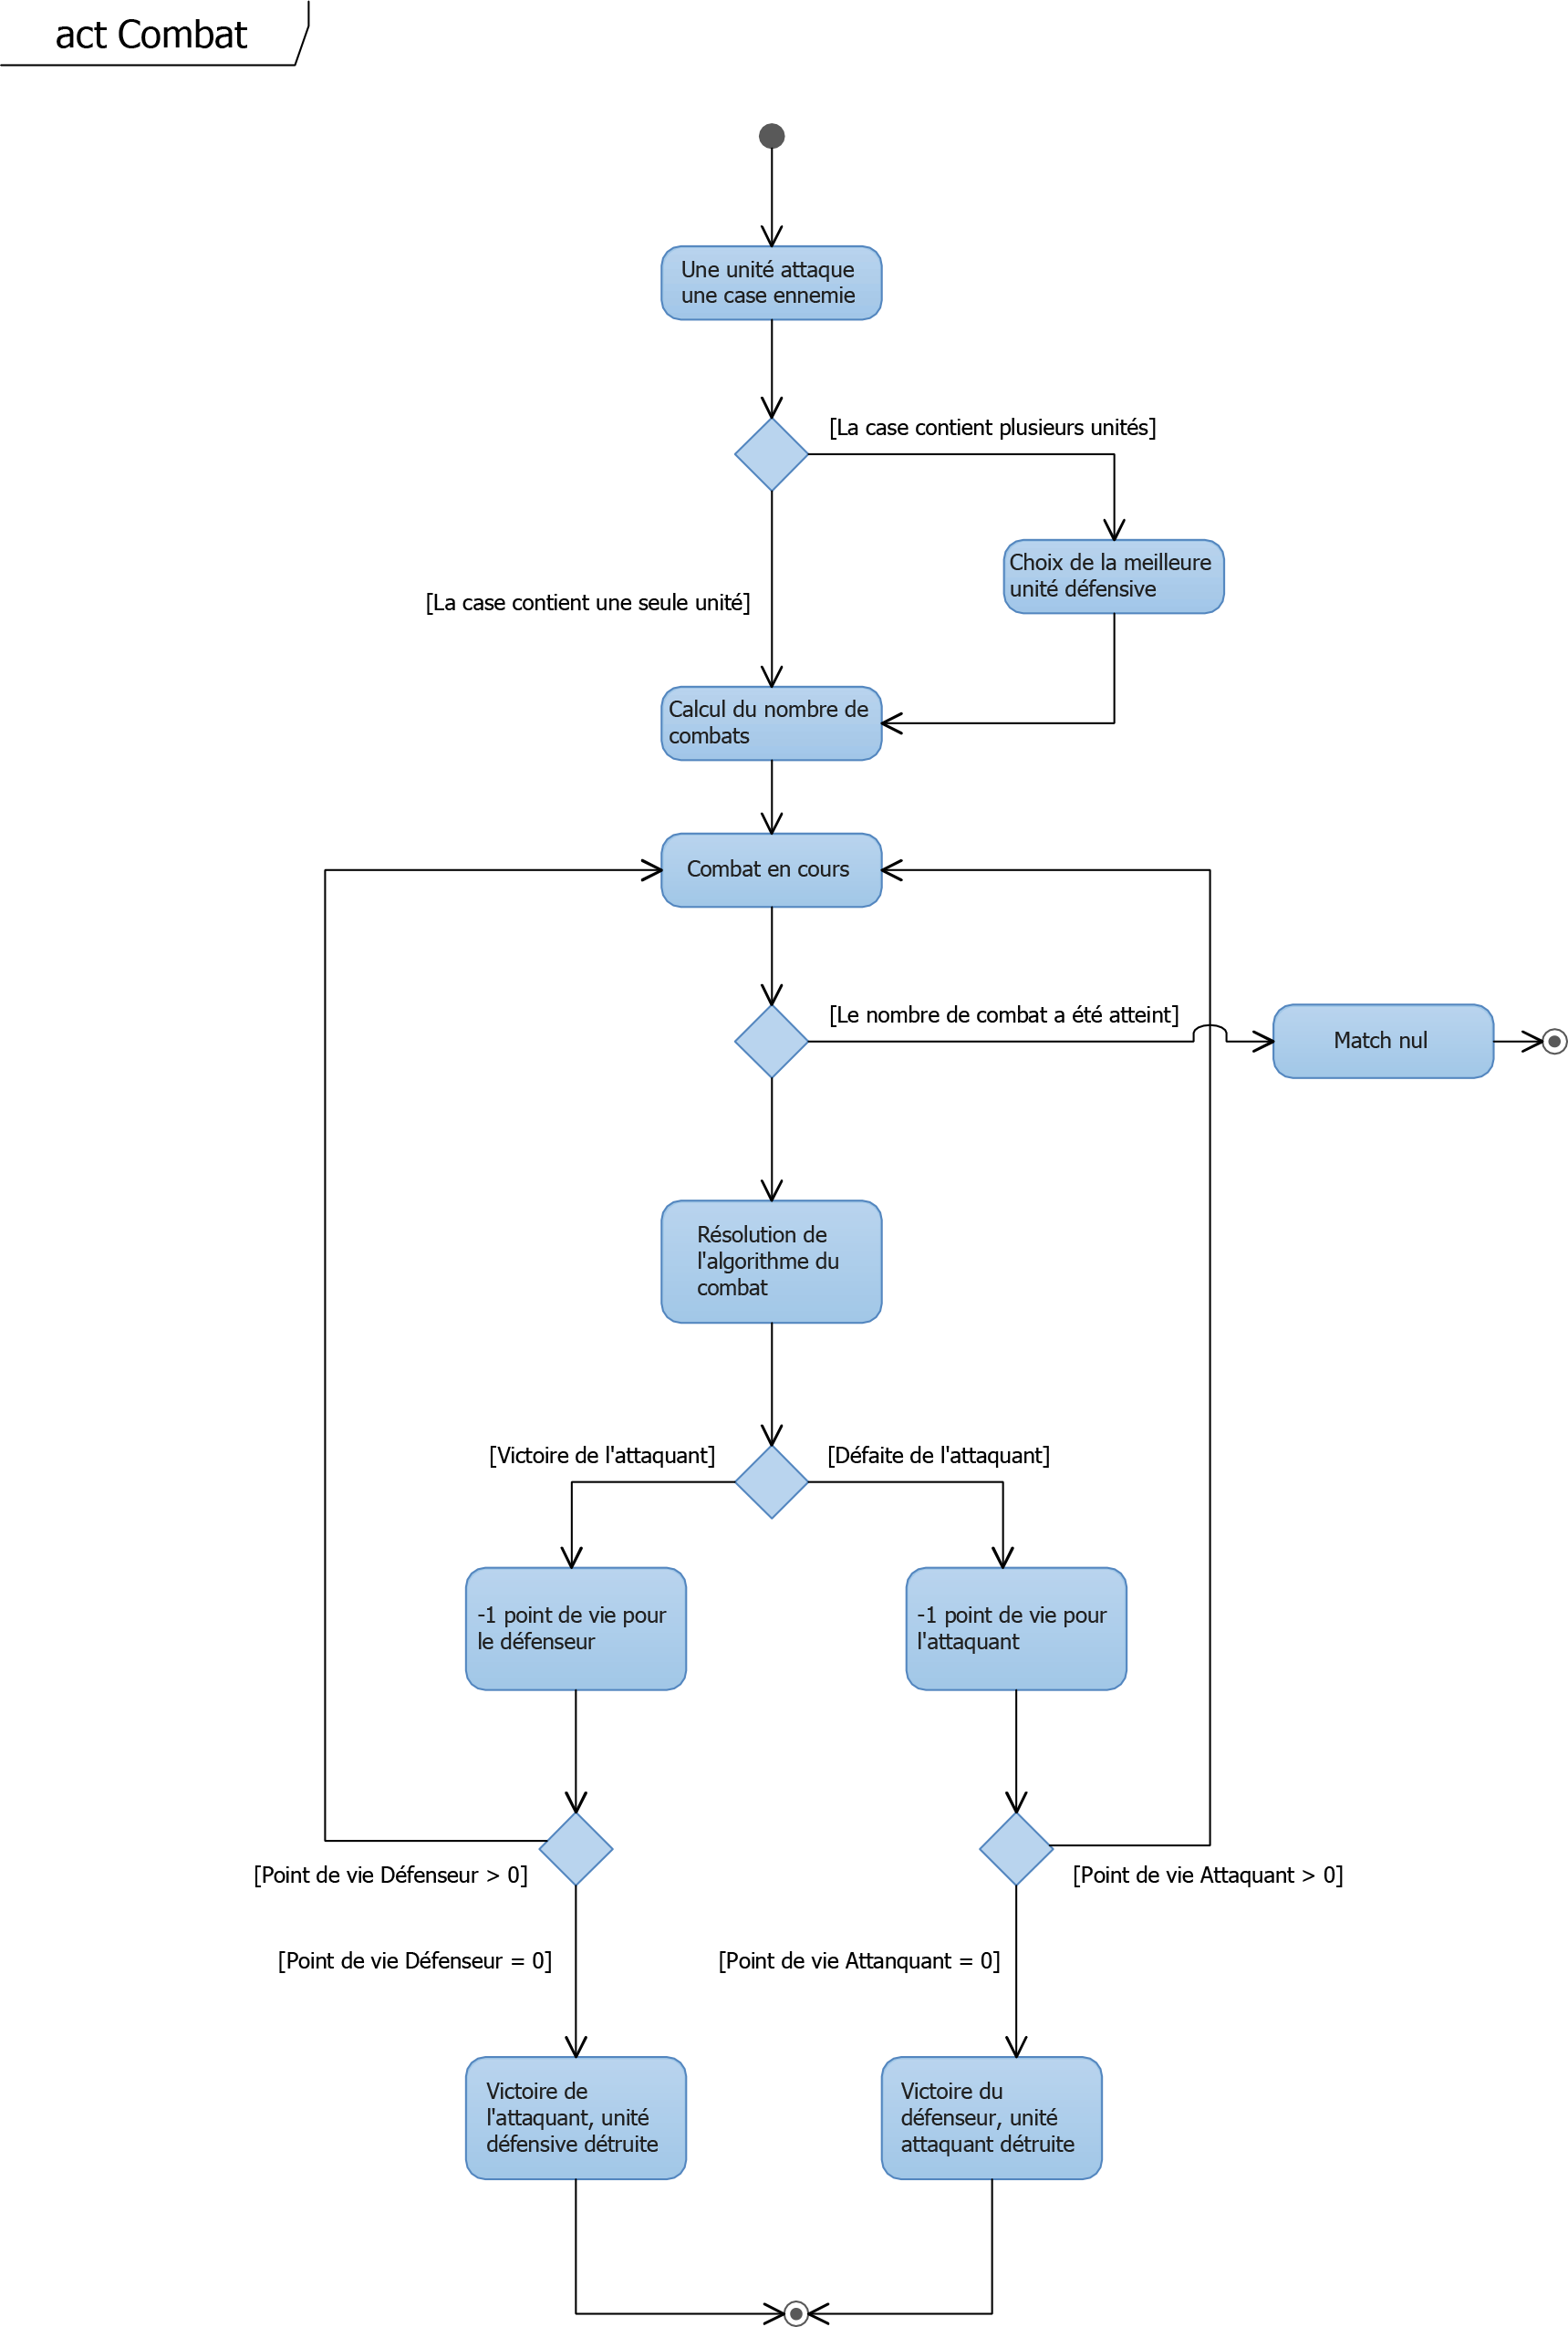
\includegraphics[height=16cm]{actCombat.png}
			\caption{Diagramme d'activité - Déroulement d'un combat}
			\label{fig:actcombat}
		\end{figure}
		\vspace*{1cm}
		Le diagramme d'activité ci-dessus (\textsc{Figure \ref{fig:actcombat}}) illustre le processus du déroulement d'un combat. Une unité attaque une case ennemie, si cette case contient plusieurs unités, on choisit la meilleure unité défensive puis on calcule aléatoirement le nombre de combat. On rentre ensuite dans le processus du combat. Tant que le nombre de combat déterminé précédement n'a pas été atteint et que les deux unités ont encore des points de vie, on résout l'algorithme du combat puis l'attaquant ou le défenseur perd un point de vie.
		\newpage
		\subsubsection{Diagramme de séquence}
			\begin{figure}[ht!]
				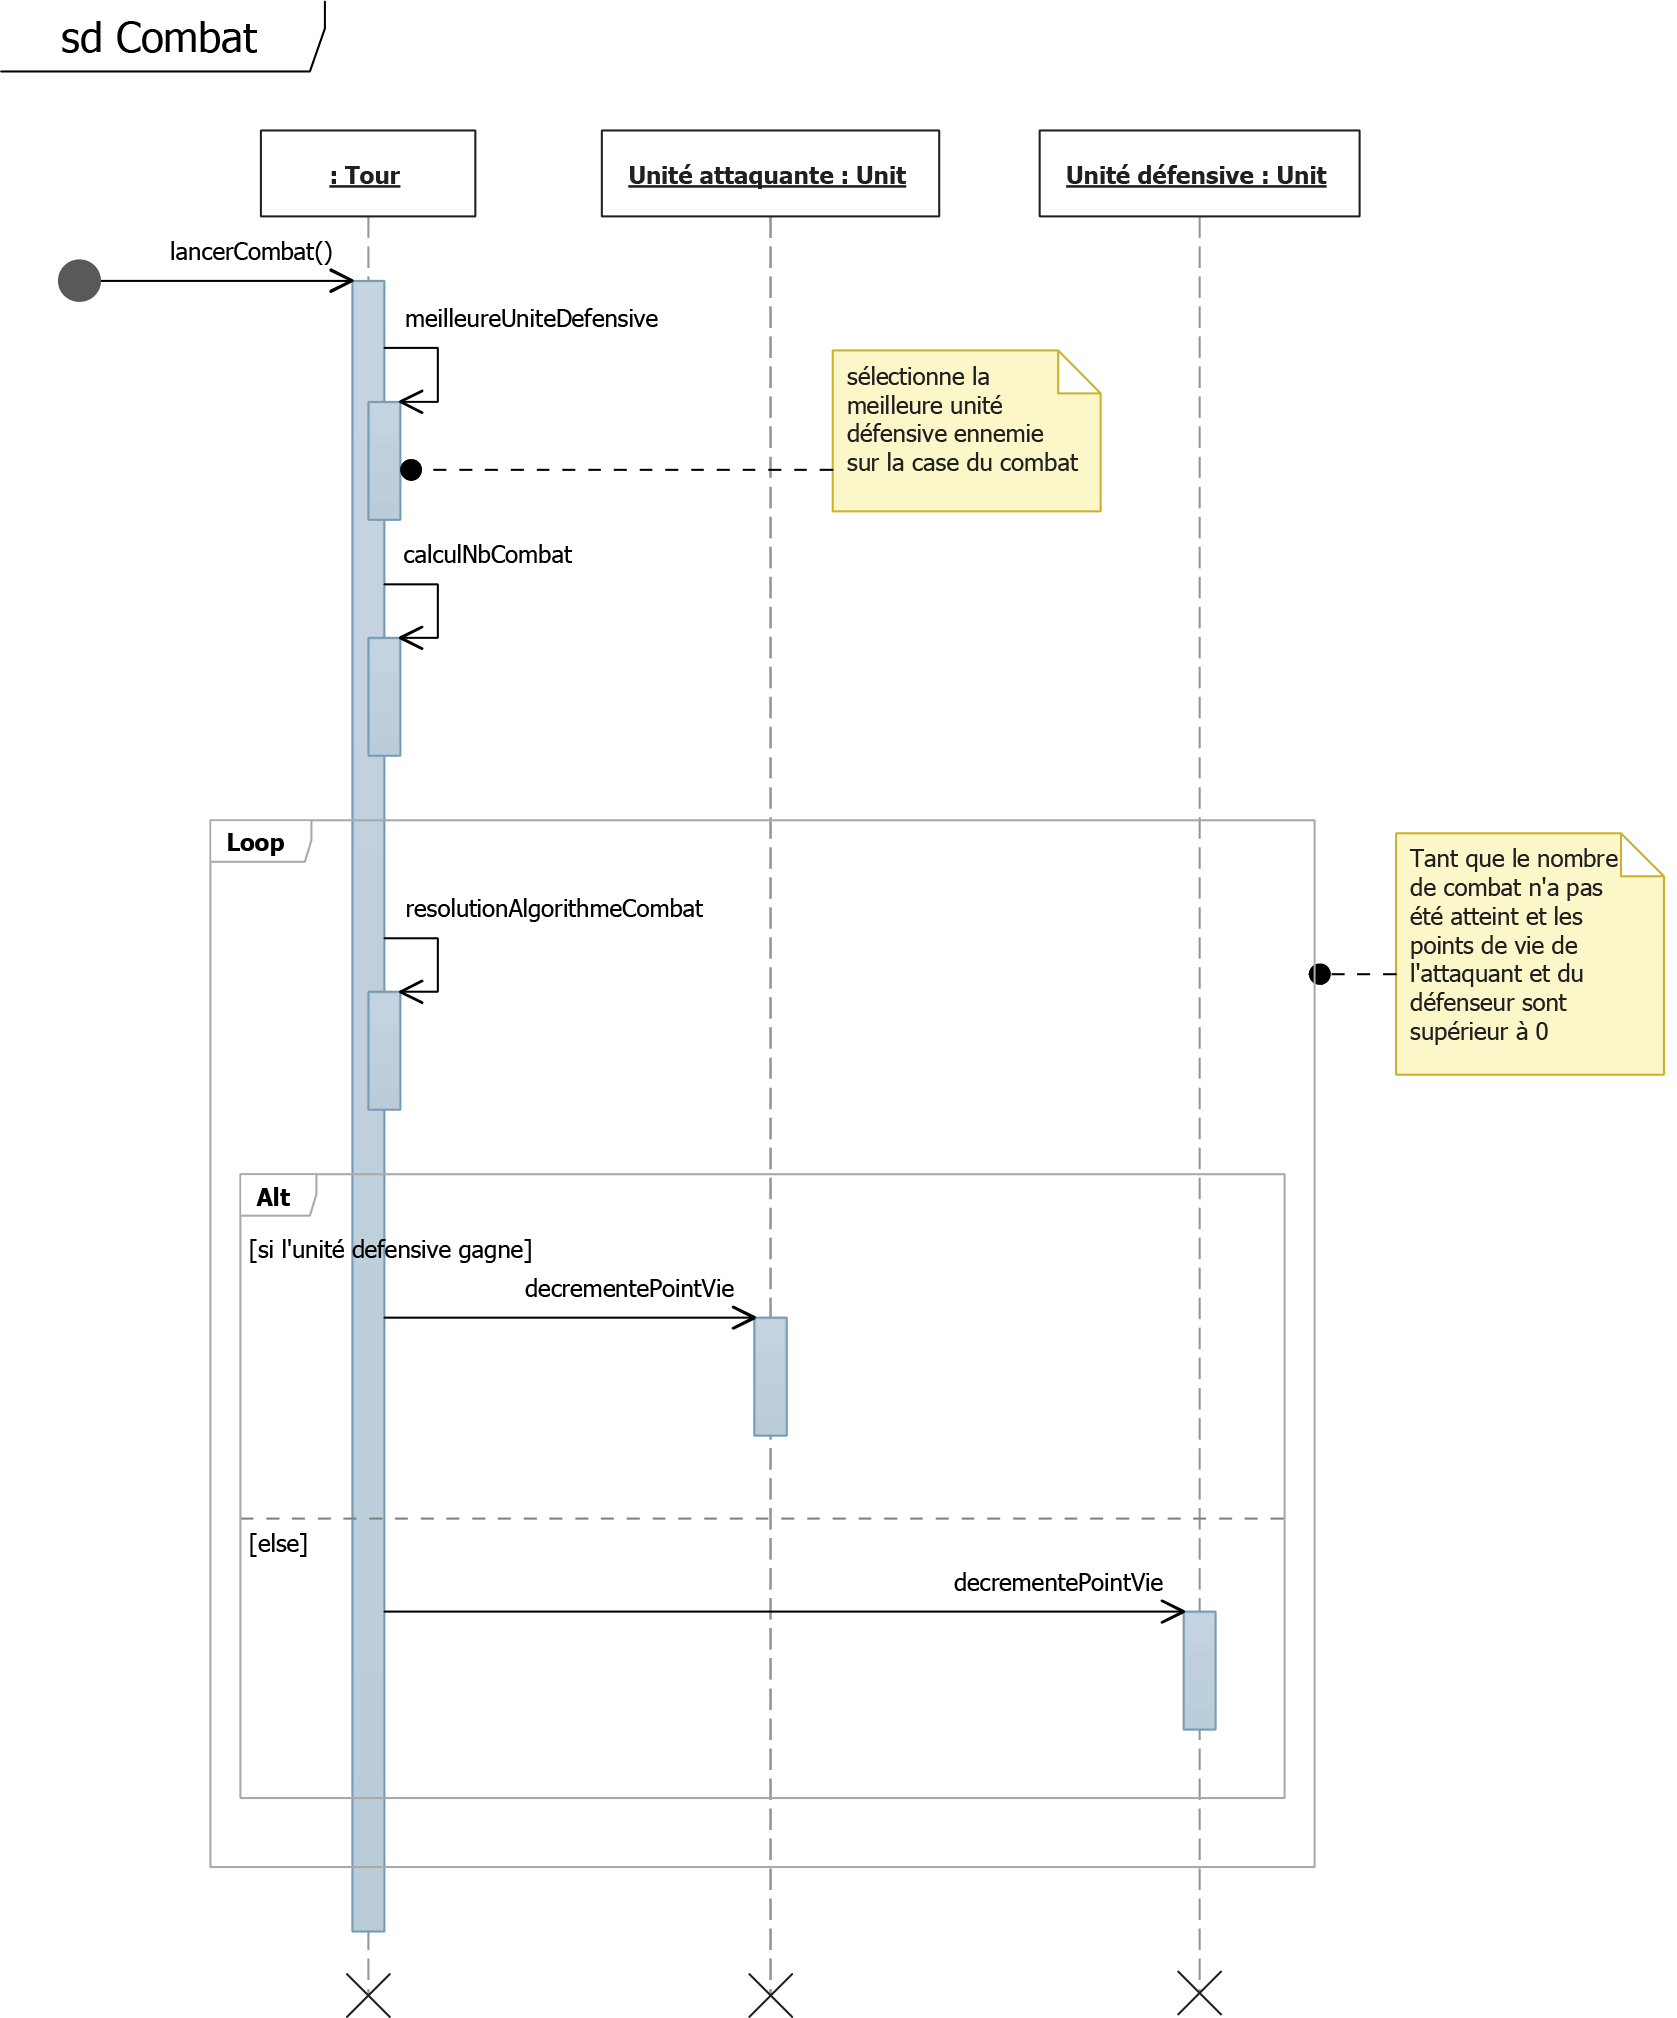
\includegraphics[height=16cm]{seqCombat.png}
				\caption{Diagramme de séquence - Déroulement d'un combat}
				\label{fig:seqcombat}
			\end{figure}
			\vspace*{1cm}
			Le diagramme d'activité ci-dessus (\textsc{Figure \ref{fig:seqcombat}}) illustre le processus du déroulement d'un combat. Une unité attaque une case ennemie, si cette case contient plusieurs unités, on choisit la meilleure unité défensive puis on calcule aléatoirement le nombre de combat. On rentre ensuite dans le processus du combat. Tant que le nombre de combat déterminé précédement n'a pas été atteint et que les deux unités ont encore des points de vie, on résout l'algorithme du combat puis l'attaquant ou le défenseur perd un point de vie.

\section{Diagramme de classe}
	\vspace*{0.5cm}
	\lipsum[1]
	\vspace*{0.5cm}
	\begin{figure}[ht!]
		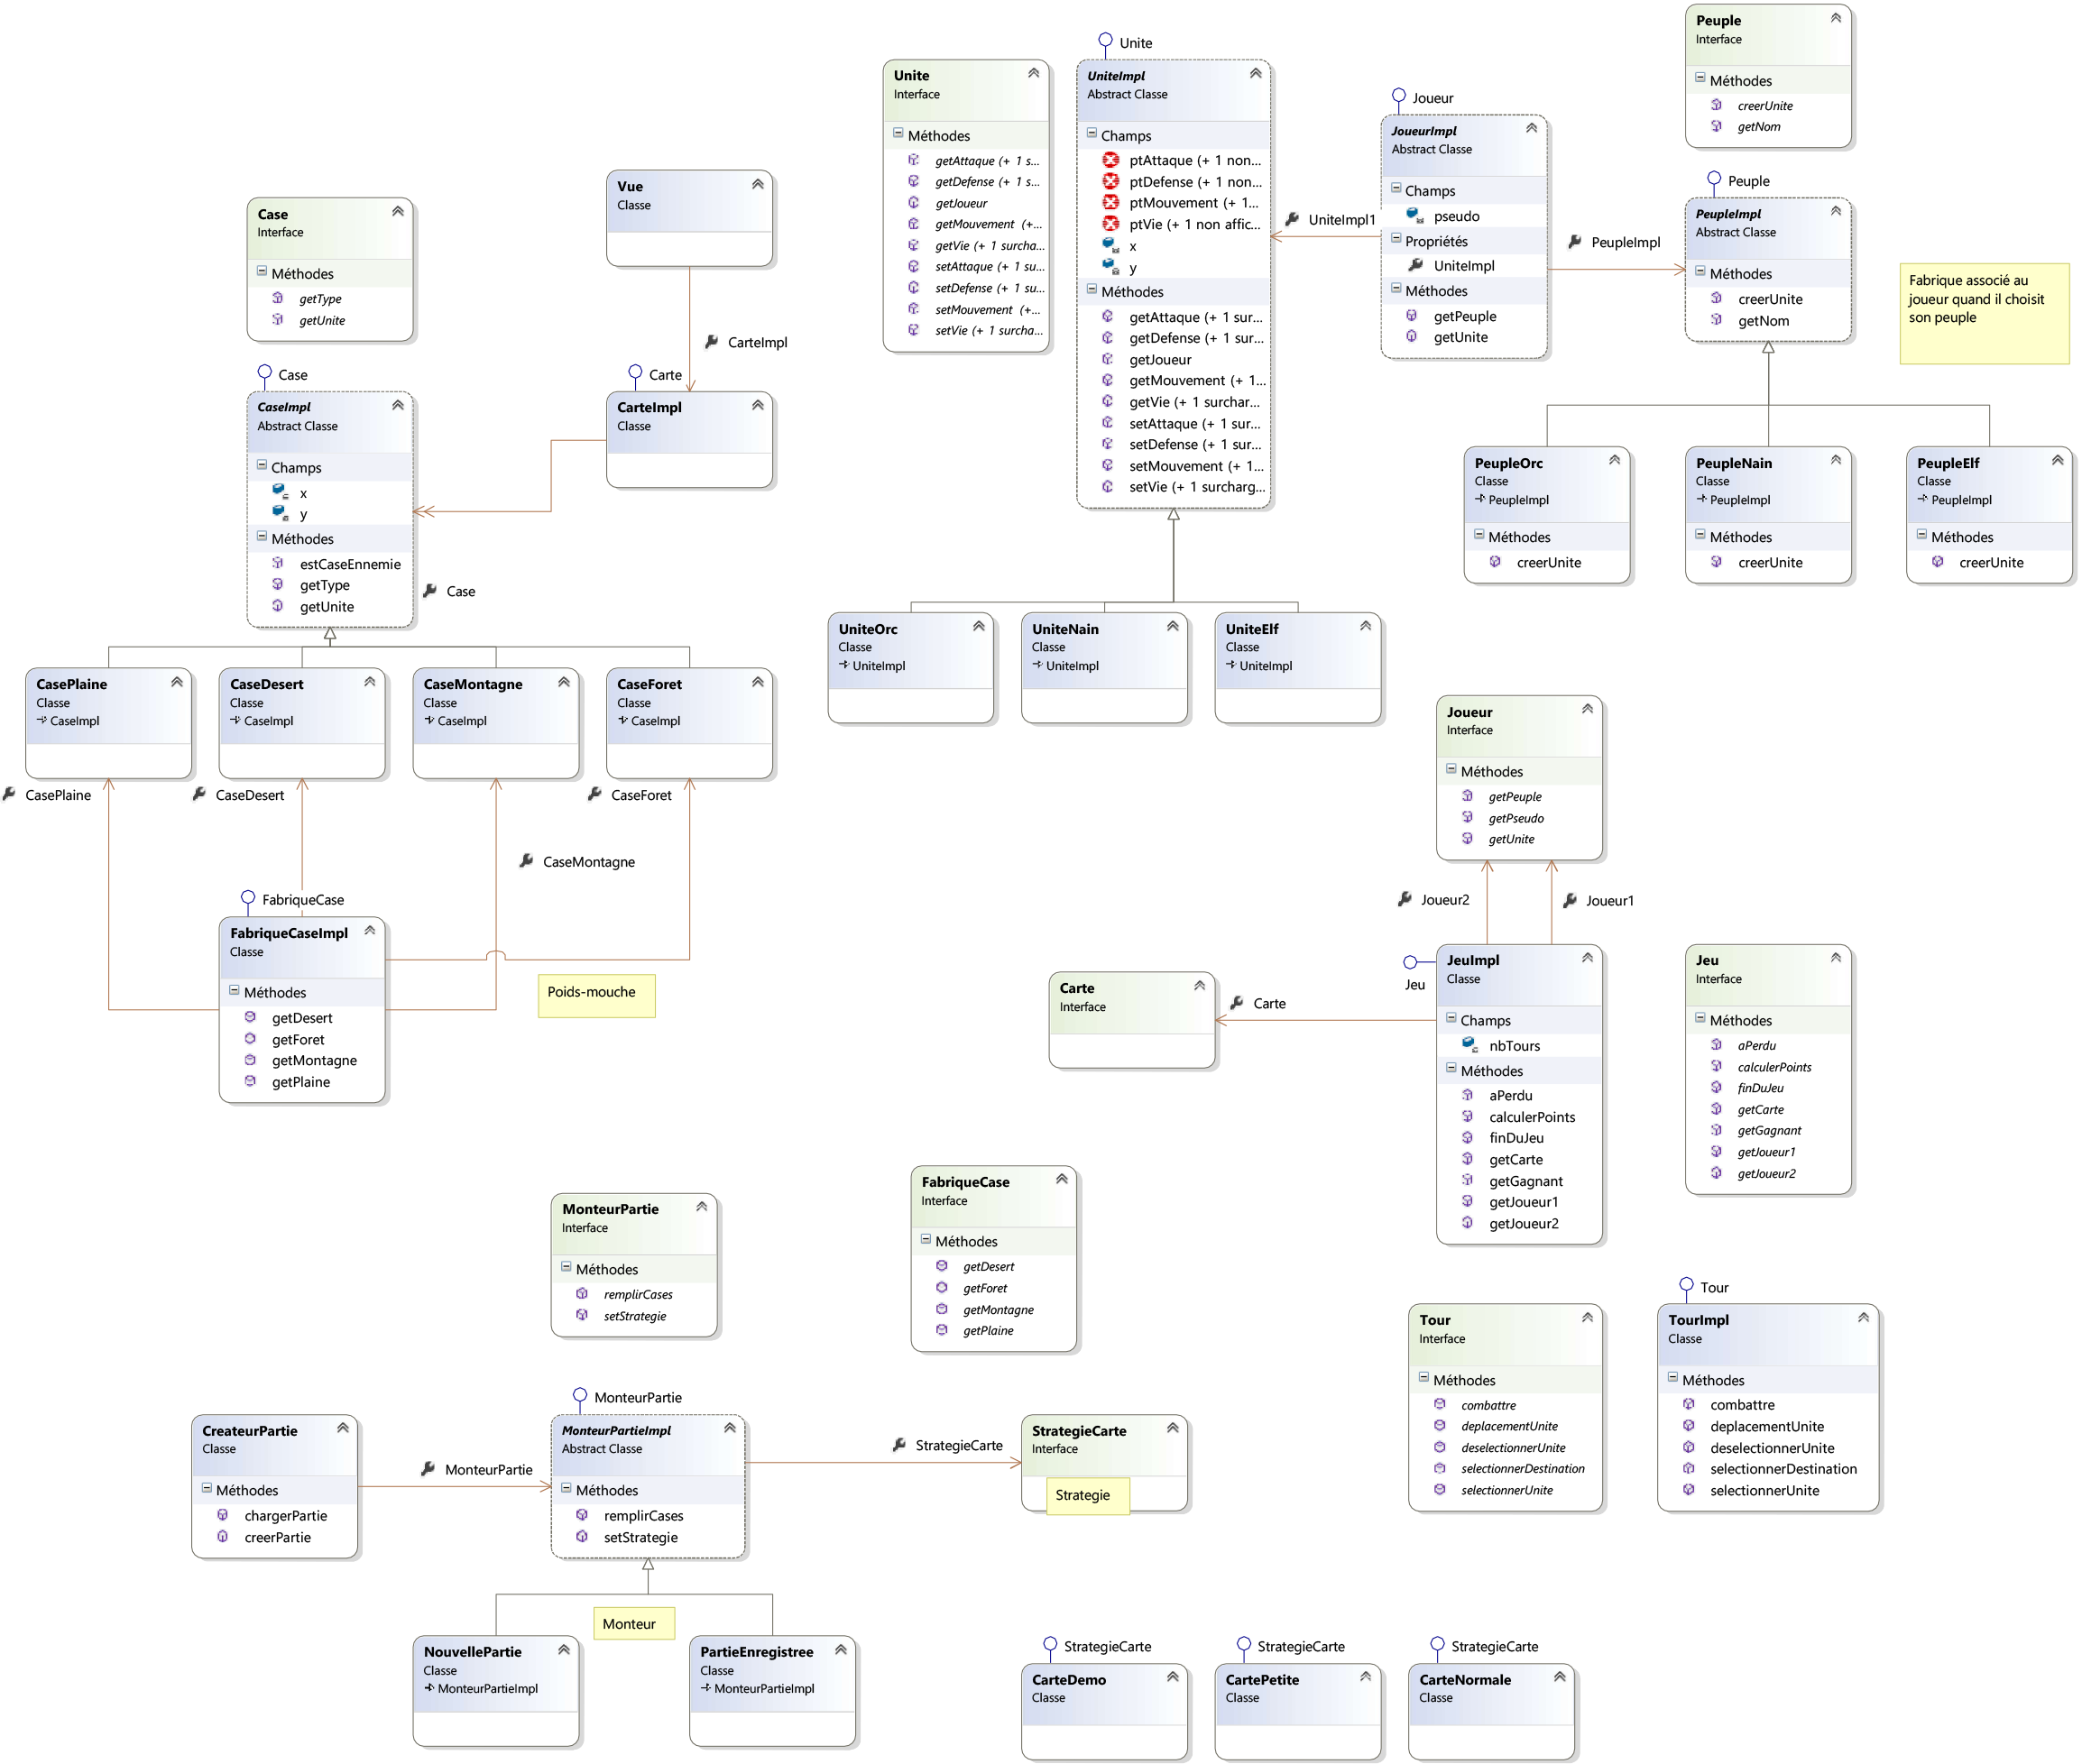
\includegraphics[height=13cm,width=15cm]{classe.png}
		\caption{Diagramme de classe - Modélisation globale}
		\label{fig:classe}
	\end{figure}
	\newpage

	\subsection{Fabrique}
		\begin{figure}[ht!]
			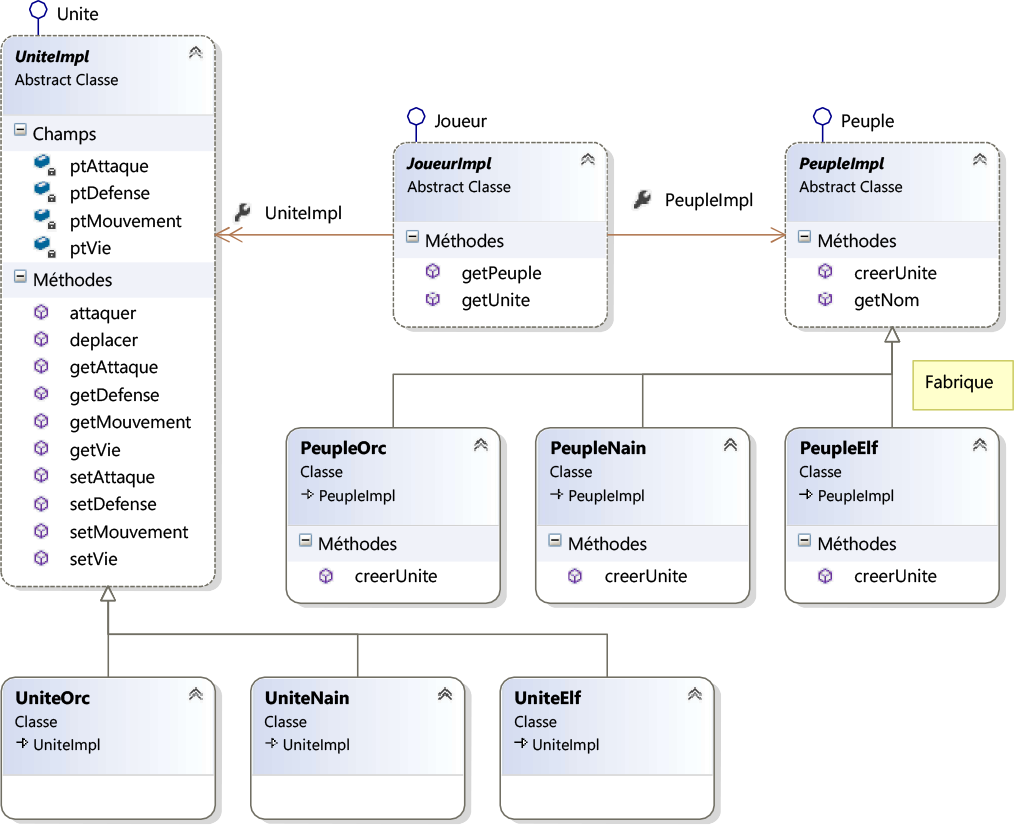
\includegraphics[height=12cm,width=14cm]{fabrique.png}
			\caption{Diagramme de classe - Fabrique}
			\label{fig:fabrique}
		\end{figure}
		\vspace*{1cm}
		\lipsum[1]
		\newpage

	\subsection{Monteur}
		\begin{figure}[ht!]
			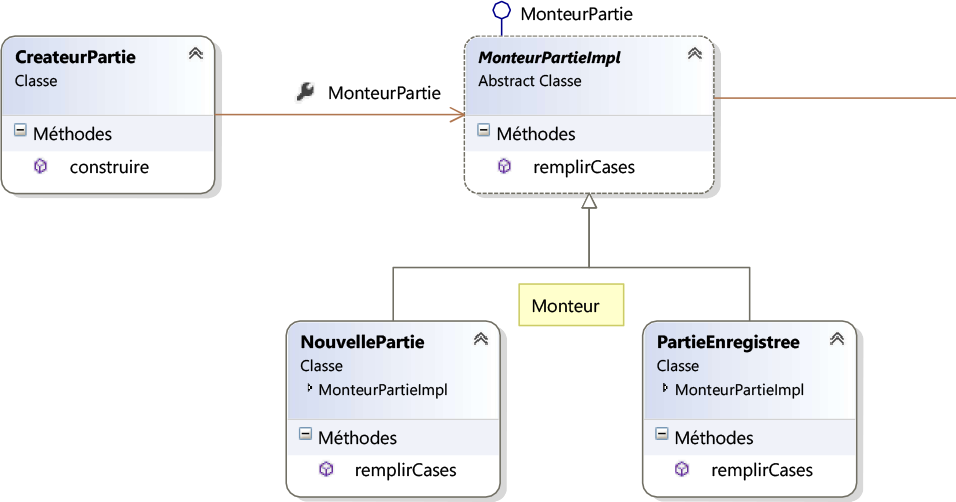
\includegraphics[height=9cm,width=14cm]{monteur.png}
			\caption{Diagramme de classe - Monteur}
			\label{fig:monteur}
		\end{figure}
		\vspace*{1cm}
		\lipsum[1]
		\newpage

	\subsection{Poids-mouche}
		\begin{figure}[ht!]
		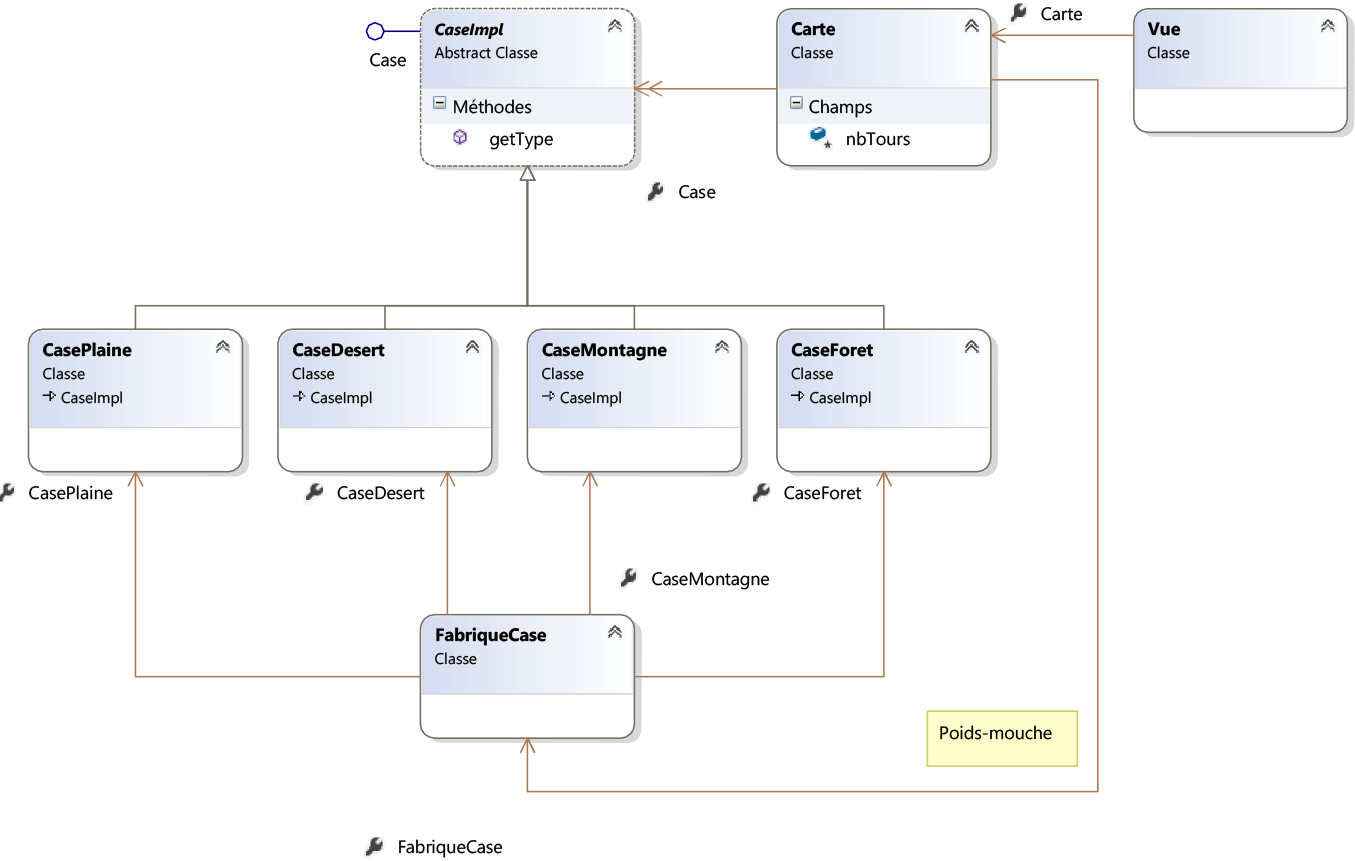
\includegraphics[height=12cm,width=15cm]{poidmouche.png}
		\caption{Diagramme de classe - Poids-mouche}
		\label{fig:poidmouche}
		\end{figure}
		\vspace*{1cm}
		\lipsum[1]
		\newpage

	\subsection{Stratégie}
	\begin{figure}[ht!]
		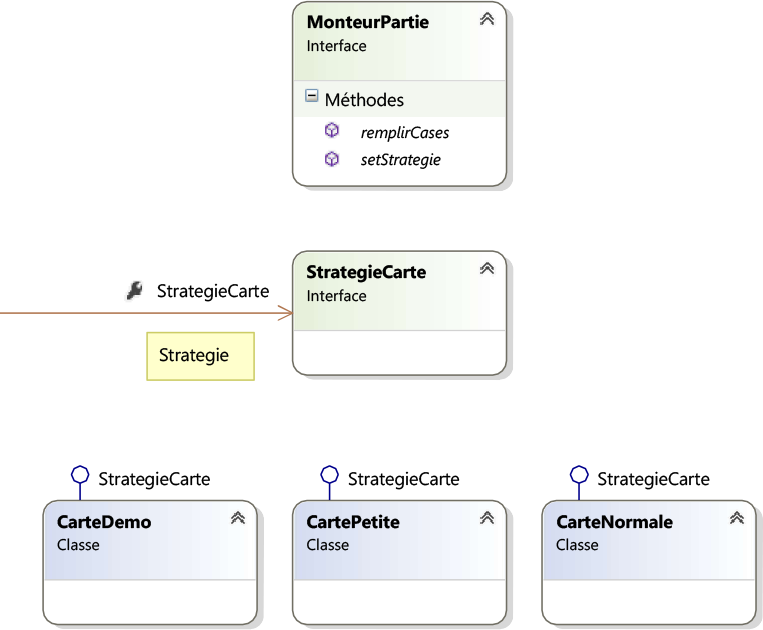
\includegraphics[height=8cm,width=10cm]{strategie.png}
		\caption{Diagramme de classe - Stratégie}
		\label{fig:strategie}
	\end{figure}
	\vspace*{1cm}
	\lipsum[1]
	\newpage

\section*{Conclusion}
	\addcontentsline{toc}{section}{Conclusion}
	\lipsum[1-2]
	\newpage
	\listoffigures

\end{document}